% Created 2015-10-16 Fri 09:57
\documentclass{scrartcl}
\usepackage[utf8]{inputenc}
\usepackage[T1]{fontenc}
\usepackage{fixltx2e}
\usepackage{graphicx}
\usepackage{longtable}
\usepackage{float}
\usepackage{wrapfig}
\usepackage{soul}
\usepackage{textcomp}
\usepackage{marvosym}
\usepackage{wasysym}
\usepackage{latexsym}
\usepackage{amssymb}
\usepackage{hyperref}
\tolerance=1000
\usepackage[margin=18mm]{geometry}
\usepackage{amsmath}
\usepackage{graphicx}
\usepackage{gensymb}
\usepackage{subfigure}
\usepackage{parskip}
\usepackage{standalone}
\usepackage{tikz,pgf,pgfplots}
\usetikzlibrary{decorations.pathmorphing,patterns}
\usetikzlibrary{arrows,snakes,backgrounds,patterns,matrix,shapes,fit,calc,shadows,plotmarks,decorations.markings,datavisualization,datavisualization.formats.functions,intersections,external}
\usetikzlibrary{decorations.pathmorphing,patterns}
\pgfplotsset{compat=1.9}
\newcommand*{\mexp}[1]{\ensuremath{\mathrm{e}^{#1}}}
\newcommand*{\laplace}[1]{\ensuremath{\mathcal{L} \{#1\}}}
\newcommand*{\laplaceinv}[1]{\ensuremath{\mathcal{L}^{-1} \{#1\}}}
\newcommand*{\realpart}[1]{\ensuremath{\operatorname{Re}(#1)}}
\newcommand*{\impart}[1]{\ensuremath{\operatorname{Im}(#1)}}
\newcommand*{\vsp}[1]{\rule{0pt}{#1}}
\newcommand*{\tderiv}[1]{\ensuremath{\frac{d^{#1}}{dt^{n}}}}
\newcommand*{\bbm}{\begin{bmatrix}}
\newcommand*{\ebm}{\end{bmatrix}}
\newcommand*{\obsmatrix}{\mathcal{O}}
\newcommand*{\contrmatrix}{\mathcal{C}}
\newcommand*{\cwh}{\ensuremath{\cos \omega h}}
\newcommand*{\swh}{\ensuremath{\sin \omega h}}
\providecommand{\alert}[1]{\textbf{#1}}

\title{Computerized control - homework 4}
\author{Kjartan Halvorsen}
\date{Due 2015-10-09}
\hypersetup{
  pdfkeywords={},
  pdfsubject={},
  pdfcreator={Emacs Org-mode version 7.9.3f}}

\begin{document}

\maketitle


\section{PID tuning}
\label{sec-1}

  Your task in this homework is to find parameters for the PID controller 
  \[ u(t) = K_p\left(e(t) + \frac{1}{T_i}\int^te(\tau)d\tau + T_d\frac{de(t)}{dt} \right). \]

  Consider the continuous-time system with transfer function
  \[ G(s) = \frac{\mexp{-0.2s}}{s+2} \]
  
  Use Ziegler-Nichols tuning (ultimate-sensitivity method). In this method, one determines the critical gain of pure proportional control of the system. That means, to determine the value of $K$ for which the closed loop system below gives self-sustained oscillations.
  \begin{center}
  \includestandalone[mode=buildnew]{feedbackK}
  \end{center}
\subsection{Analytical solution}
\label{sec-1-1}

  Determine the ultimate gain by calculations. 
\begin{enumerate}
\item Determine the frequency $\omega_p$ for which the nyquist curve for $G(s)$ crosses the negative real axis. That is, solve for $\omega$ in 
     \[ \arg G(i\omega) = -\pi. \]
     Actually, this leads to a transcendental equation. You can solve this numerically using, for example, the function \texttt{fsolve} in matlab.
\item Determine the gain $K=K_u$ such that the nyquist curve for the open loop system $KG(s)$ passes through the point $(-1,0)$.
\end{enumerate}

  This will give you the ultimate gain $K_u$ and period of the oscillations $T_u$ needed to apply the tuning rules.
\subsection{Determine by simulation}
\label{sec-1-2}

\begin{enumerate}
\item Use matlab (or simulink) to implement the system. To define the transfer function of the plant you can do

\begin{verbatim}
s = tf('s');
G = exp(-0.2*s)/(s+2)
\end{verbatim}
\item Plot a Bode diagram using \texttt{margin(G)}. Verify that the phase curve crosses $-180\degree$ at the frequency $\omega_p$ that you determined in the previous exercise. Include the bode-diagram in your report.
\item Define the closed loop system with proportional feedback, $K$.
\item Simulate step-responses for various values of the gain $K$. Increase  $K$ until the system shows sustained (neither increasing nor decaying) oscillations. Note the corresponding value, $K_u$ and the period of the oscillations, $T_u$. Verify that they are the same as (or close to) the values you determined analytically. Include a figure of the step-response for critical gain $K_u$ to your report (plot showing 10-20 periods of oscillations).
\end{enumerate}
 
 
\subsection{Implement a PID-controller}
\label{sec-1-3}

   Use Table 8.3 in Å\&W to determine the parameters $K_p$, $T_i$ and $T_d$ based on $K_u$ and $\omega_p$. 
\begin{enumerate}
\item Implement the (continuous-time) controller and the closed loop system.
\item Plot the Bode diagram for the closed-loop system and include in your report. What is the bandwidth of the closed-loop system?
\item Plot the Bode diagram and Nyquist diagram for the open-loop system $F(s)G(s)$. What is the phase marginal? Include a figure (Bode or Nyquist) in your report, where you indicate the phase marginal.
\item Simulate a step response for the closed-loop system and include in your report. You will probably need to use a Padé-approximation of the delay. To get an LTI-system with approximated delays use \texttt{Gcp = pade(Gc, 4)} for a 4th order Padé approximation. What is the overshoot of the step response in percent of the final value?
\end{enumerate}
\section{Solution}
\label{sec-2}
\subsection{Analytical solution}
\label{sec-2-1}

\begin{enumerate}
\item The equation to solve to find the phase-crossover frequency is
      \[ \arg G(i\omega) = -\pi. \]
      Write this as
      \[ \arg \mexp{-0.2i\omega} - \arg (i\omega + 2) + \pi = 0, \]
      or 
      \[ -0.2\omega - \atan \frac{\omega}{2} + \pi = 0. \]
      This can be solved in matlab with the line
      \texttt{fsolve(inline('-atan2(x,2) - 0.2*x + pi'), 0)} and gives the answer
      \[\omega_p = 8.953. \]
\item The phase-crossover frequency is the frequency for which the Nyquist curve crosses the negative real axis. Multiplying $G(i\omega)$ with a real, positive gain $K$ does not change the phase and so the phase-crossover frequency remains the same. $KG(i\omega)$ will cross the negative real axis at $\omega_p$. To find the ultimate gain $K_u$ that will cause the Nyquist curve to pass throgh the point (-1,0), solve
      \[ |K_uG(i\omega_p)| = 1, \]
      which lead to
      \[ K_u = \frac{1}{|G(i\omega_p)|} = \frac{|i\omega_p + 2|}{|\mexp{-0.2i\omega_p}|} = \sqrt{\omega_p^2 + 4} \approx 9.174. \]
\end{enumerate}
   
\subsection{Simulation}
\label{sec-2-2}

   Here is example matlab-code for generating the model and simulating a step:

\begin{verbatim}
T = 0.2;
s = tf('s');
G = exp(-s*T) / (s+2)
Ku = 1/abs(evalfr(G, i*wp))
Gc = feedback(Ku*G, 1);
step(Gc)
\end{verbatim}
     The figure below shows the first five seconds of the step response. Clearly, the period of the oscillations is $T_u = 0.702$.
   
      \begin{center}
      \includestandalone[mode=buildnew, width=0.6\linewidth]{ultimate_gain_experiment}
      \end{center}

   Bode-diagram of open-loop transfer function with ultimate gain (using \texttt{margin})
      \begin{center}
      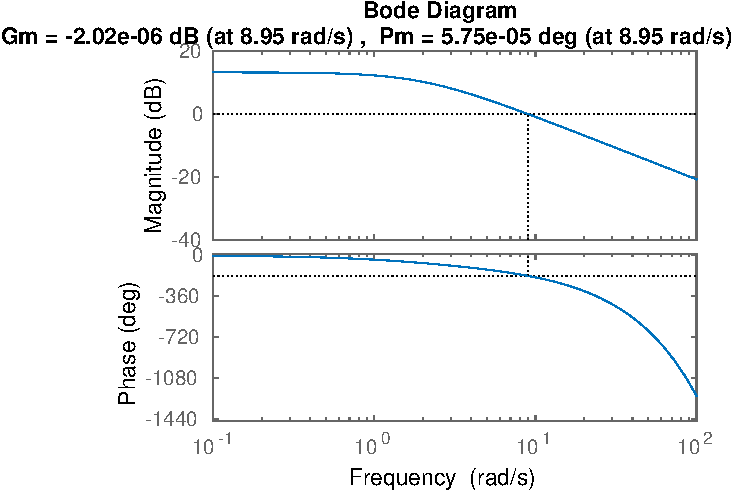
\includegraphics[width=0.6\linewidth]{ultimate_margin-crop}
      \end{center}

  
\subsection{Implement PID}
\label{sec-2-3}

   Using table 8.3 from Å\&W we obtain the PID controller with parameters
   \begin{align*}
   K_p &= 0.6 K_u = 5.5\\
   T_i &= 0.5T_u = 0.35\\
   T_d &= T_u/8 = 0.088
   \end{align*}

   The Bode diagram of the closed loop system with the PID controller is given below.
      \begin{center}
      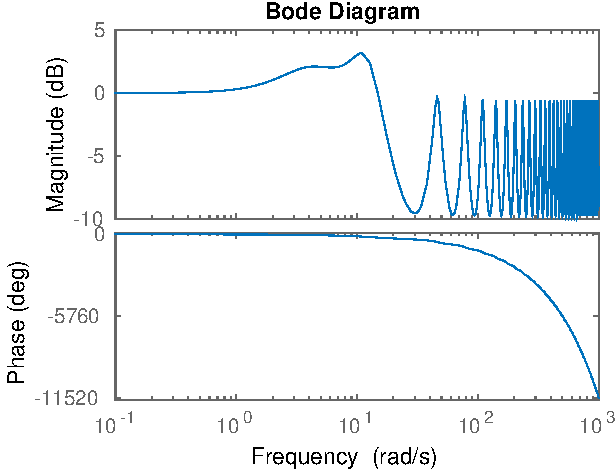
\includegraphics[width=0.6\linewidth]{pid_gc_bode-crop}
      \end{center}
   The closed-loop system has bandwidth 17.2 rad/s.

   The Bode diagram of the open-loop system shows a phase margin of 46.4 degrees:
      \begin{center}
      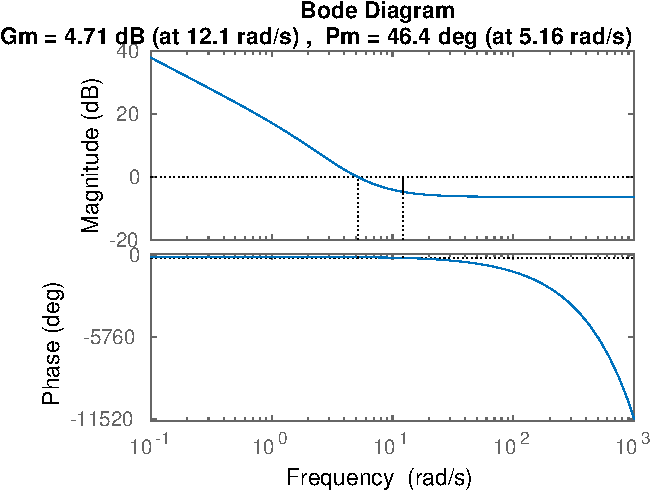
\includegraphics[width=0.6\linewidth]{pid_go_margin-crop}
      \end{center}

    With a padé approximation of the delay, the step response of the closed loop system is given below
      \begin{center}
      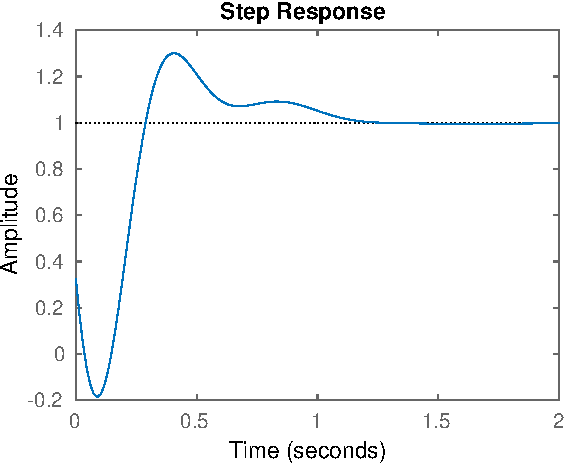
\includegraphics[width=0.6\linewidth]{pid_step_pade-crop}
      \end{center}
    The initial response of the close-loop system before the delay of the open-loop system is due to the approximation. It should be exactly zero. The overshoot is about 30\%.

\end{document}
